\part{Unit 1: Fundamentals of Ethical Hacking}
\section{Introduction and Virtual Machines}

The Cybersecurity Specialist course aims to train professionals in the field of information security. These individuals will possess strong technical skills, providing added value to companies in the fight against cybercrime. The course is divided into three units:
\begin{enumerate}
    \item \textbf{Unit 1} focuses on the theoretical prerequisites and technical skills necessary for an Ethical Hacker. It covers topics such as networking, operating systems, and an introduction to programming;
    \item \textbf{Unit 2} centers on the phases of Penetration Testing, exploring the tools and techniques used by hackers in the real world;
    \item \textbf{Unit 3} provides students with a comprehensive understanding of how to monitor security events, manage ongoing attacks, and adopt best practices at the enterprise level to minimize the impact on business activities.
\end{enumerate}

In the past century, computing and the web were primarily the domain of experts, including hackers. The term \emph{hacker}, often associated with digital piracy, encompasses three distinct types of hackers:
\begin{itemize}
    \item \textbf{White Hat Hackers}, also known as "Ethical Hackers," operate with a strict adherence to ethical standards. Their work involves improving security with the consent of the system owner;
    \item \textbf{Grey Hat Hackers} operate in a legal and ethical gray area. They often act without the owner's permission but with the intent of improving security. While their actions can uncover vulnerabilities, they can also be controversial and sometimes illegal;
    \item \textbf{Black Hat Hackers} are criminals who break into computer networks with malicious intent. They may deploy malware to destroy files, steal information, hold computers hostage, or pilfer passwords, credit card numbers, and other personal data. Their motivations are typically opportunistic, such as financial gain. Stolen data is often sold on the dark web, where items like credit card details, online payment system access, medical records, and even streaming service accounts are traded.
\end{itemize}

An Ethical Hacker is a cybersecurity expert capable of simulating cyber-attacks to identify potential vulnerabilities in a company's systems. These simulations, known as \emph{Penetration Tests}, are crucial for detecting and fixing security issues in digital networks, software, and devices, thereby protecting enterprises and public entities from cybercriminal activities. Key responsibilities of an Ethical Hacker include:
\begin{itemize}
    \item Conducting penetration tests on IT infrastructures and web applications;
    \item Ensuring the security of sensitive and private data, such as payment details, login credentials, and passwords.
\end{itemize}

It is crucial to emphasize that penetration testing should only be performed with the formal consent of the system or network owner. Conducting such tests without permission is illegal and can lead to severe legal consequences.


\subsection{Virtualization Process}
Virtual machines (VMs) are emulations of computer systems that provide the functionality of a physical computer. They run on a physical host machine and are managed by a virtualization layer. The process of creating and managing VMs is known as virtualization (\Cref{fig:virtualization}).
Virtualization involves several key steps:

\begin{enumerate}
    \item \textbf{Hypervisor Installation:} The hypervisor, also known as the Virtual Machine Monitor (VMM), is installed on the host machine. The hypervisor can be of two types:
    \begin{itemize}
        \item \textbf{Type 1 (Bare Metal):} Runs directly on the host's hardware.
        \item \textbf{Type 2 (Hosted):} Runs on top of an existing operating system.
    \end{itemize}
    \item \textbf{Resource Allocation:} The hypervisor allocates resources (CPU, memory, storage, and network) from the physical host to each VM.
    \item \textbf{VM Creation:} Virtual machines are created by defining their virtual hardware specifications (number of CPUs, amount of memory, disk size, etc.).
    \item \textbf{Operating System Installation:} An operating system is installed on the virtual machine, just as it would be on a physical machine.
    \item \textbf{VM Management:} The hypervisor manages the execution of VMs, handles resource allocation dynamically, and ensures isolation between VMs.
\end{enumerate}

\begin{figure}
    \begin{center}
        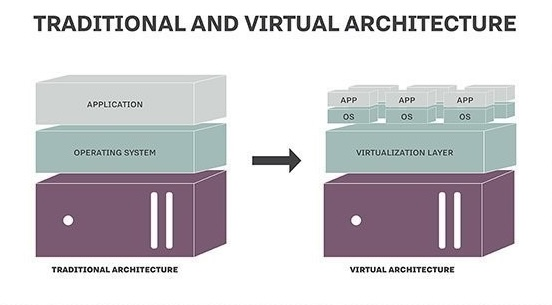
\includegraphics[width=\textwidth]{images/virtualization.jpg}
        \caption{Traditional vs Virtual architecture.}
        \label{fig:virtualization}
    \end{center}
\end{figure}


\subsubsection{Virtual Hardware}
A virtual machine emulates physical hardware components such as:
\begin{itemize}
    \item \textbf{CPU:} Virtual CPUs (vCPUs) are assigned to the VM by the hypervisor.
    \item \textbf{Memory:} Virtual memory is allocated from the host's physical memory.
    \item \textbf{Storage:} Virtual disks are created using files on the host's storage system.
    \item \textbf{Network:} Virtual network interfaces connect VMs to the host's network and to other VMs.
\end{itemize}

\subsubsection{Hypervisor Role}
The hypervisor plays a critical role in:
\begin{itemize}
    \item \textbf{Resource Management:} Dynamically allocating resources to VMs based on their needs.
    \item \textbf{Isolation:} Ensuring that each VM operates independently and securely.
    \item \textbf{Efficiency:} Optimizing resource usage to maximize the performance of VMs.
\end{itemize}

\subsubsection{Execution Flow}
The execution flow of a VM includes:
\begin{enumerate}
    \item \textbf{Boot Process:} The VM goes through a boot process similar to a physical machine, loading its operating system from the virtual disk.
    \item \textbf{Application Execution:} Applications run within the VM, utilizing the virtualized hardware.
    \item \textbf{Hypervisor Interaction:} The VM interacts with the hypervisor for tasks like I/O operations, which the hypervisor translates to the physical hardware.
\end{enumerate}

\subsubsection{Benefits of Virtualization}
Virtualization offers several advantages:
\begin{itemize}
    \item \textbf{Cost Efficiency:} Reduces the need for physical hardware.
    \item \textbf{Scalability:} Easily create, modify, and delete VMs as needed.
    \item \textbf{Isolation:} Provides a secure and isolated environment for each VM.
    \item \textbf{Resource Utilization:} Maximizes the usage of physical resources.
\end{itemize}

Virtualization is a powerful technology that enables the efficient use of hardware resources, providing flexibility, scalability, and isolation. Virtual machines are an integral part of modern computing environments, supporting a wide range of applications from development to production systems.
